\section{Hyperparameter} \label{hyperparam}

Hyperparameter sind die Parameter, die zur anfänglichen Konfiguration des neuronalen Netzes als auch zur Konfiguration des Lernprozesses heran gezogen werden. Um im Laufe der Arbeit verstehen zu können, wie die Objektdetektoren auf Seiten der Netzarchitektur und des Lernverhaltens optimiert wurden, ist demnach ein kurzer Einblick in den Themenbereich der Hyperparameter von Nöten.

\subsection*{Anzahl der LTUs}
Die Anzahl der LTUs im ANN ist dafür ausschlaggebend, wie hoch der Komplexitätsanspruch eines Klassifizierungsproblems sein darf, um noch vom ANN gelöst werden zu können. Die Anzahl der LTUs hängt hauptsächlich von den Eingangsdaten ab. Über die optimalste Anzahl an LTUs pro Schicht lässt sich allerdings nur schwer etwas vorhersagen. Generell gilt, dass bei gleicher Anzahl an LTUs tiefere Netze eine weitaus höheren Parametereffizienz aufweisen als breitere Netze, da diese schneller gegen den gewünschten Zustand konvergieren. Zudem lassen sie sich somit schneller und kostengünstiger trainieren. So müssten bei einem 2x32 Netz 1024 Gewichtungen angepasst werden, während es bei einem 32x2 Netz dies nur 128 sind \cite{AurelienGeron.2018}.

\subsection*{Initialisierung der Gewichtungen}
Auch stellt die Initialisierung der Gewichte eines ANNs zu Beginn des Trainingsprozesses eine berechtigte Frage dar. Falls keine bereits trainierten ANNs für ein Klassifikationsproblem vorliegen, so werden die Gewichtungen meist zufällig nach einer Normalverteilung gewählt \cite{AurelienGeron.2018}. 

Dies hat allerdings zur Folge, dass nach der Berechnung der gewichteten Summen aller LTUs die Gewichtungswerte der folgenden Schicht nicht mehr normalverteilt sind, da für die Varianz zweier unkorrelierter Zufallsvariablen das Superpositionsprinzip

\begin{equation} \label{varianz}
Var(X + Y) = Var(X) + Var(Y)
\end{equation}
\equations{Superpositionsprinzip anhand der Varianz}

gilt.

Durch die größer werdende Standardabweichung können demnach Gewichtungswerte entstehen, die weit vom Mittelwert Null abweichen. Dies kann wiederum dazu führen, dass der Gradientenabstieg während des Backpropagation-Verfahrens nur langsam vollzogen werden kann, da der Gradient bei bestimmten Aktivierungsfunktionen wie der \textit{Sigmoid-Funktion} gegen Null konvergiert \cite{AurelienGeron.2018}. 

Eine \textit{Xavier Initialisierung} umgeht das Problem der sogenannten \textit{schwindenden Gradienten}, indem die Gewichte nach

\begin{equation} \label{xavier}
W \sim U[-\frac{\sqrt{6}}{\sqrt{n_{j} + n_{j+1}}},\frac{\sqrt{6}}{\sqrt{n_{j} + n_{j+1}}}]
\end{equation}
\equations{Standardverteilung nach Xavier Initialisierung}

gleichverteilt werden, wobei $n_{j}$ die Anzahl an LTUs der $j-ten$ Schicht sind \cite{XavierGlorot.2010}.

\subsection*{Anzahl an Epochen}

Die Anzahl der Epochen beschreibt die Durchläufe durch einen bestimmten Trainingsdatensatz während der Trainingsphase. Ist die Anzahl zu hoch gewählt, wird Gefahr gelaufen, sogenanntes \textit{Overfitting} des ANNs zu erreichen. Dies bedeutet ein fehlendes Abstraktionsvermögen des ANNs durch Auswendiglernen der Trainingsdaten zu erreichen und damit alleinig eine richtige Erkennung der Trainingsdatensätze zu ermöglichen.  

\subsection*{Lernrate}

Die Lernrate $\eta$ (\ref{gradientenverfahren}) gibt an, wie groß die Sprünge sein sollen und damit indirekt wie viele Iterationen benötigt werden, um das Minimum der Kostenfunktion zu erreichen. Ziel der Anpassung einer Lernrate ist es, mit möglichst wenig Iterationen und Testdaten die optimale Konstellation des neuronalen Netzes zu berechnen. Deshalb wird sie standardmäßig zu Beginn der Iterationen groß gewählt, um sich dem Minimum schnell zu nähern, während sie am Ende immer kleiner gewählt wird, um nicht über das globale Minimum hinaus zu gehen. Dieses Vorgehen wird als \textit{Simulated Annealing} bezeichnet, während das Funktion zum Festlegen der Lernrate als \textit{Learning Schedule} betitelt wird \cite{AurelienGeron.2018}.

Die Anzahl der Durchläufe wird zu Beginn des Verfahrens zunächst hoch angesetzt, das Verfahren wird aber genau dann gestoppt, sobald der Gradientenvektor unter eine gewisse Abbruchgrenze fällt. Zwar ist das globale Minimum zu diesem Zeitpunkt noch nicht erreicht, allerdings kann es auch nie vollkommen erreicht werden, da die für das Gradientenverfahren genutzten Aktivierungsfunktionen nie einen partiellen Ableitungswert gleich Null zulassen \cite{AurelienGeron.2018}. In diesem Sinne wird auch von \textit{Toleranz} gesprochen.

\subsection*{Moment}

Das Gradientenverfahren kann beschleunigt werden, indem während des Gradientenabstiegs frühere Gradienten Einfluss auf den nächsten Gradientenschritt nehmen. Es wird ein \glqq Momentum\grqq{} aufgebaut. Damit das Momentum 

\begin{equation} \label{momentum}
\begin{split}
m_x = \beta \cdot m_{x-1} + \eta\frac{\partial E}{\partial w_{ij}} \\
w_{ijt} = w_{ijt-1} - m 
\end{split}
\end{equation}
\equations{Momentum Optimierung}

allerdings nicht zu groß wird, beschränkt der Hyperparameter $\beta \in [0,1]$ die Größe des Momentums \cite{AurelienGeron.2018}.

Die Momentum Optimierung kann dazu benutzt werden, das \textit{stochastische Gradientenverfahren} bzw. \textit{Mini-Batch} Verfahren zu beschleunigen und lokale Minima besser zu überwinden.

\subsection*{Auswahl des Gradientenverfahrens}

Generell wird zwischen drei verschiedenen Arten unterschieden, das Gradientenverfahren durchzuführen (siehe Abbildung \ref{gradient}):

\begin{figure}[ht]
	\begin{center}
		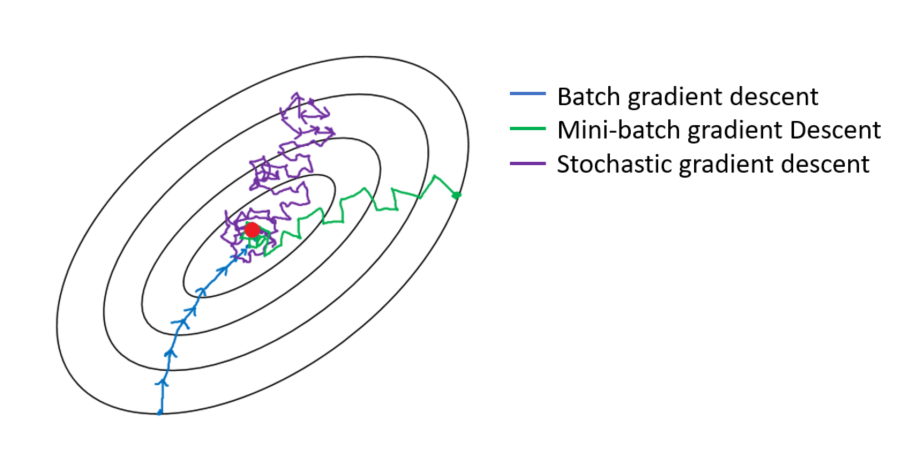
\includegraphics[width=15cm]{Bilder/gradient_descent.png} 
		\caption[Gradientenverfahren]{Gradientenverfahren \cite{ImadDabbura.20171221}}
		\label{gradient}
	\end{center}
\end{figure}

Beim \textit{Batch} Verfahren werden in einem Trainingsdurchlauf, der \textit{Epoche}, alle vorhandenen Daten des Trainingsdatensatzes herangezogen, um einen Gradientenabstieg zu vollziehen. Dies ist bei großen Trainingsdatensätzen auffällig langsam, dafür aber hinsichtlich der Erreichung des lokalen Minimums sehr zielstrebig \cite{AurelienGeron.2018}.

Das \textit{stochastische Gradientenverfahren} führt nach jedem einzelnen Dateneintrag im Trainingsdatensatz einen Gradientenabstieg durch. Da nur wenige Daten des ANNs verändert werden müssen, ist dieses Verfahren deutlich schneller, dafür aber unregelmäßiger hinsichtlich der Erreichung des Minimums. Oft wird das stochastische Gradientenverfahren verwendet, wenn nicht der komplette Trainingsdatensatz in den Hauptspeicher oder Grafikspeicher geladen werden kann. Diese Fähigkeit wird oft als \textit{Out-of-Core} Fähigkeit bezeichnet. Es hat auch den Vorteil, besser das globale Minimum der Kostenfunktion aufzufinden, da bei lokalen Minima die Chance besteht, durch den unregelmäßigen Gradientenabstieg das lokale Minimum wieder zu überwinden \cite{AurelienGeron.2018}.

Ein Kompromiss der beiden Verfahren bietet das \textit{Mini-Batch} Verfahren, bei dem wiederholt Teilmengen des gesamten Datensatzes für einen Gradientenabstieg verwendet werden. Die Anzahl an Elementen einer solchen Teilmenge wird als \textit{Batch Größe} bezeichnet. Genauso wie das \textit{Batch} Verfahren bietet das \textit{Mini-Batch} Verfahren den Vorteil, die partiellen Ableitungen als Matrizenoperationen auf die Grafikkarten auszulagern, um die Performanz durch Parallelisierung zu steigern. Zusätzlich muss weniger Speicher für einen Gradientenabstieg reserviert werden \cite{AurelienGeron.2018}.

\subsection*{Aktivierungsfunktionen}

Zwei bekannte und ähnliche Aktivierungsfunktionen sind die \textit{Sigmoid-Funktion} und die \textit{Tangens Hyperbolicus} Funktion. Da diese allerdings durch ihr schnelles Konvergieren gegen den Grenzwert anfällig für das Problem \textit{schwindender Gradienten} sind \cite{AurelienGeron.2018}, wird die \textit{Rectified Linear Unit} (ReLU) bzw. \textit{Parametric/Leaky Rectified Linear Unit} (PReLU/LRelU) Aktivierungsfunktion bevorzugt (siehe Abbildung \ref{relu}). 

\begin{figure}[ht]
	\subfigure[RELU]{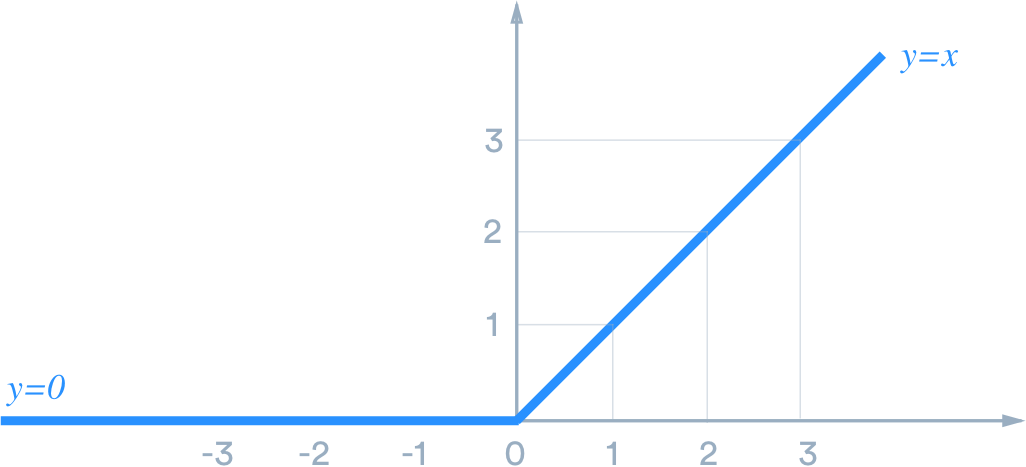
\includegraphics[width=7.5cm]{Bilder/relu.png}} 
	\subfigure[PReLU/LReLU]{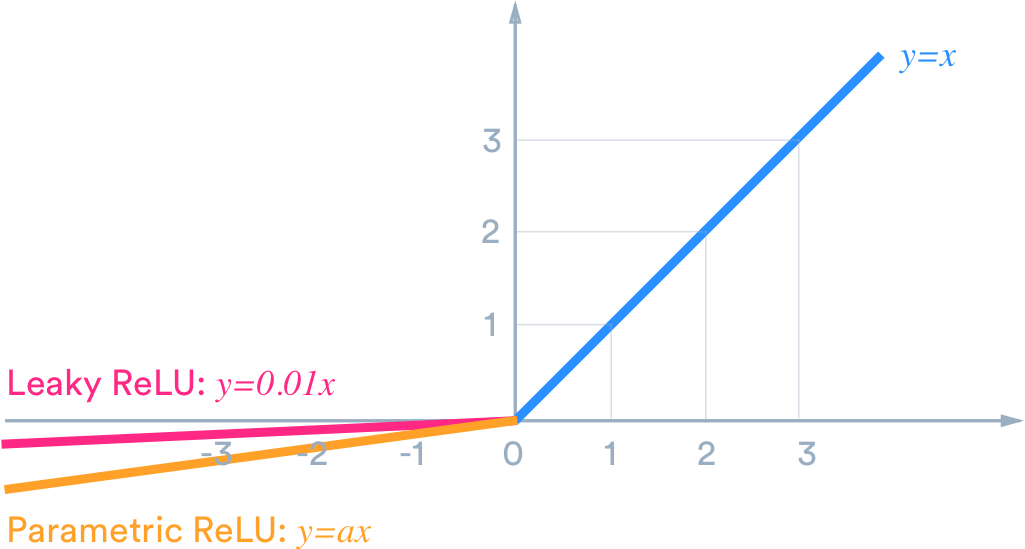
\includegraphics[width=7.5cm]{Bilder/prelu.png}} 
	\caption[ReLU-Aktivierungsfunktionen]{ReLU-Aktivierungsfunktionen \cite{DanqingLiu.20171130}} 
	\label{relu}
\end{figure} 

Bei ReLU kann es während des Trainingsprozesses dazu kommen, dass LTUs nach dem Gradientenabstieg einen negativen Wert aufweisen, weshalb sie nicht weiter aktiviert werden und für den Rest der Trainingsdauer \glqq tot\grqq{} sind. Um dies zu verhindern, wurde \textit{LReLU} dazu genutzt, um eine Reaktivierung zu ermöglichen, da auch für negative LTU Werte ein Gradient der Aktivierungsfunktion bestimmt werden kann. Bei \textit{LReLU} ist die Steigung der Funktion im zweiten Quadranten statisch gewählt, während sie bei \textit{PReLU} dynamisch von neuronalen Netz während des Trainingsprozesses selbst gelernt werden kann \cite{AurelienGeron.2018}.

Eine letzte Variante der Aktivierungsfunktionen beschreibt die \textit{ELU} Funktion (siehe Abbildung \ref{elu}).

\begin{figure}[ht]
	\begin{center}
		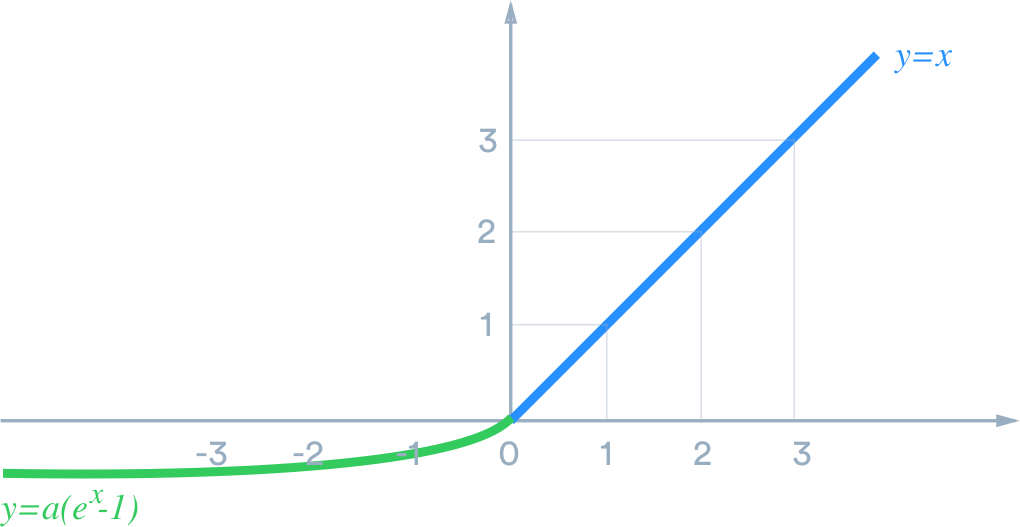
\includegraphics[width=12cm]{Bilder/elu.png} 
		\caption[ELU-Aktivierungsfunktion]{ELU-Aktivierungsfunktion \cite{DanqingLiu.20171130}}
		\label{elu}
	\end{center}
\end{figure}

Sie besitzt nicht nur die Eigenschaft schwindende Gradienten und damit nicht anpassbare, sogenannte \glqq tote\grqq{} LTUs zu verhindern, sondern ist im gesamten Definitionsbereich ebenso eine stetig differenzierbare Funktion, was das Gradientenverfahren beschleunigt. Als Standardwert für den Streckungsfaktor $\alpha$ der niederen Funktion wird oft Eins verwendet. Nachteil der \textit{ELU} Funktion ist der erhöhte Rechenaufwand, was aber durch die schnellere Konvergenz kompensiert wird \cite{AurelienGeron.2018}.

